
\chapter{解决方案}
\label{chap:contribute}

在这个网络如此发达,web2.0和云计算的使用日益普及的时代,人们的文档管理方式也发生了巨大的改变。但是由于种种原因,有些好的模式和方法并没有被高校用户所认可与广泛使用。而且可以证实,有些公共网络上的文档服务也并不适合高校用户。所以就导致了大部分高校用户的个人文档管理方式依然停留在10年前的单机模式下,也就势必带来本文上一章所提到的诸多文档管理的问题。而本文描述系统的设计目标就是帮助高校用户解决这些问题。本章下面就针对上面提到的每一个问题逐一提出本系统的解决方案。

\section{文档写作解决方案}
\label{sec:write}

\subsection{LaTex}
\label{sec:latex}

上一章提到,高校用户文档写作过于依赖Word软件,带来的诸多弊端。但是,在很多人看来Word依然是用来写文档的绝佳选择。在我国,Word的普及率如此之高,它有的时候甚至会被认为是编辑文档的唯一选择。仅“所见即所得”一项,Word就会赢得绝大多数用户的心。但是很多人也许不知道,在国外,对于写学术报告和科技论文,有更加标准也更加普及的编辑工具,那就是\LaTeX,世界上很多著名的出版机构斗接受或强制要求作者使用\LaTeX稿件,接受 LaTeX 稿件的出版社大都有自己的文稿样式模板,主要就是一个类型文件包,简称类包。如果稿件未被甲出版社采用,在转投乙出版社前,只需将稿件第一句中类包名称由甲出版社的改为乙出版社的,整篇稿件的样式就随之自动转换过来了,确实很方便。国外知名大学也大多都要求学生使用\LaTeX编写科技报告和论文,这和国内Word一家独大的局面截然不同。本系统用来解决文档编辑问题的基础之一就是\LaTeX。那么什么是\LaTeX呢?

\LaTeX是一种排版系统,它基于\TeX\footnote{国计算机教授高德纳在1978年编写的功能强大的排版软件,高德纳最早开始自行编写它的原因是当时十分粗糙的排版水平已经影响到他的巨著《计算机程序设计艺术》(The Art of Computer Programming)的印刷质量。他以典型的黑客思维模式,最终决定自行编写一个排版软件。}排版系统并由此发展而来。它是由美国电脑学家莱斯利·兰伯特在20世纪80年代初期开发,利用这种格式,即使用户没有排版和程序设计的知识也可以充分发挥由\TeX所提供的强大功能,能在几天,甚至几小时内生成很多具有书籍品质的印刷品。对于生成复杂表格和数学公式,这一点表现得尤为突出。因此它非常适用于生成高印刷质量的科技和数学类文档。这个系统同样适用于生成从简单的信件到完整书籍的所有其他种类的文档。与其他的文字排版系统(比如Word)相比,\LaTeX最突出的优势就是高质量、高专业水准的文稿排版效果。下面简单比较一下\LaTeX和Word:
\begin{description}
\item[入门难度]  Word 特点就是“所见即所得”,其基本功能初学者很容易掌握,很多 Word 用户都是无师自通。但随着篇幅和复杂程度的增加,花费在文稿格式上的精力和时间要明显加大,如图~\ref{fig:xfig2}蓝色示意曲线所示。因为创建自定义编号、交叉引用、索引和参考文献等就不是“所见即所得”了,得耐着性子反复查阅 Word 的在线帮助或借助相关软件帮忙。
对于 \LaTeX 初学者,即就是编排很简单的文章,也要花较多的精力和时间去学习那些枯燥的命令和语法,特别是排写数学公式,经常出错,多次编译不能通过,使很多初学者望而却步。可是一旦掌握,不论文 稿长短和复杂与否都会熟练迅速地完成,先前学习 \LaTeX 的精力投入将由此得到回报,如图~\ref{fig:xfig2}红色示意曲线所示。关于\LaTeX入门难度大的问题,本系统下面介绍\smarkdown的时候会给出解决方案。
\begin{figure}[H]
  \centering
  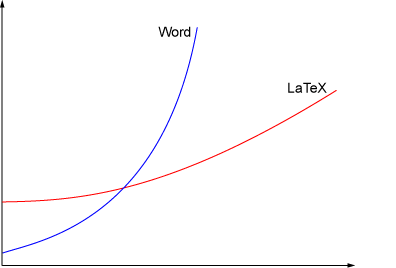
\includegraphics{latexVSword}
  \caption{latex与word的学习曲线比较}
  \label{fig:xfig2}
\end{figure}
\item[内容与格式] 当用 Word 写作时,要花很多精力对页版式、章节样式、字体属性、对齐和行距等文本参数进行反复选择对比,尤其是长篇文章,经常出现因疏忽而前后文体格式不一致的现象;当在稿件中插入或删除一章或章节次序调整时,各章节标题、图表和公式等的编号都要用手工作相应修改,稍有不慎就会出现重号或跳号。 我们既是作者又是编辑还兼排字工。

使用 \LaTeX 编版,如无特殊要求,只要将文稿的类型(article、report 或 book 等)告诉 \LaTeX,就可专心致志地写文章了,至于文稿样式的各种细节都由 \LaTeX 统一规划设置,而且非常周到细致;当修改稿件时,其中的章节、图表和公式等的位置都可任意调整,无须考虑编号,因为在源文件里就没有编号,文件中的所有编号都是在最后编译时 \LaTeX 自动统一添加的,所以绝对不会出错。
换句话说,Word 把文稿的内容与样式混为一体,而 \LaTeX 将它们分离,作者只需专注于文稿的内容,而文稿的样式几乎不用过问,\LaTeX 是你的聪明而忠诚的文字秘书,如有特殊要求,也可使用命令修改,\LaTeX 会自动将相关设置更新,无一遗漏。
\item[数学公式问题] 

Word 有个公式编辑器,可以编辑普通数学公式,但使用很不方便,外观效果较差,也不能自动编号,尤其是很难作为文本的一部分,融入某一行中,大都专起一行。如果碰到复杂的数学公式,编辑起来就很困难。有些用户只好另外安装可嵌入 Word 环境的工具软件 Math-Type 来弥补这一不足。

\LaTeX 的特长之一就是数学公式编辑,方法简单直观,“所想即所得”,公式的外观精致细腻,而且公式越复杂这一优点就越明显。普通单行公式可以像纯文字文本一样插入字里行间。下面举三个例子比较一下 ,其中图~\ref{fig:xfig3}是 DOC 格式的屏幕显示效果,图~\ref{fig:xfig4}是将 DOC 格式文件通过 Acrobat 转换为 PDF 格式的效果,图~\ref{fig:xfig5}是\LaTeX生成的PDF格式的效果,显然\LaTeX的数学公式排版效果更好。
\begin{figure}[H]
  \centering
  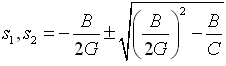
\includegraphics{wordformula}
  \caption{Word显示数学公式效果}
  \label{fig:xfig3}
\end{figure}
\begin{figure}[H]
  \centering
  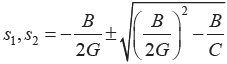
\includegraphics{wordformulapdf}
  \caption{Word转成pdf后显示数学公式效果}
  \label{fig:xfig4}
\end{figure}
\begin{figure}[H]
  \centering
  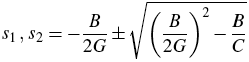
\includegraphics{latexformula}
  \caption{LaTeX里显示数学公式}
  \label{fig:xfig5}
\end{figure}
\item[参考文献] Word 目前还不具备管理参考文献的功能,用户一般都是采用 Reference Manager 或是 NoteExpress 等外部工具软件来解决这一问题。
而创建参考文献却是 \LaTeX 的强项。\LaTeX 自带一个辅助程序 BibTeX,它可以根据作者的检索要求,搜索一个或多个文献数据库,然后自动为文稿创建所需的参考文献条目列表。如果编写其它文件用到相同的参考文献时可直接引用这个数据库。参考文献的样式和排序方式都可以自行设定。很多著名的科技刊物出版社、学术组织和 TUG 网站等都提供相关的 BibTeX 文献数据库文件,可免费下载。
\item[稳定性和安全性] 一篇科技论文少则几十页,多则上百页,其中含有许多图形和公式(Word 将公式处理为图形),正是由于 Word“所见即所得”,论文中的图形都要完整地插入页面 。随着文件的篇幅增大图形数量增多,处理速度明显减慢。编写一篇论文要无数次地打开、保存和关闭,往往要长时间等待甚至死机或文稿无法打开,所以 Word 经常出现“文件恢复”提示信息,但其中的图形很有可能丢失,取而代之的是一个小红叉。如果将文件分解为多个子文件,可以缓解这一问题,但又会出现难以自动创建目录、索引和参考文献等新问题;若章节、图表和公式需要 在子文件之间调换调整,那编号就全乱套了。
\LaTeX 是纯文本文件,所有图形都是在最后编译时调入。同一篇文章,其 \LaTeX 源文件只有 Word 文件尺寸的几十分之一。所以,\LaTeX 源文件的长短,不会对文件存取和编辑过程产生明显影响。\LaTeX 也允许采用多个子文件,章节和图表可随意增删,\LaTeX 是在最后编译时才将所有子文件汇总排序,生成统一的文件页码、标题序号、图表和公式编号以及各种目录。
Word 从问世到现在不断地更新版本,并经常要求下载补丁程序,防止病毒攻击。\LaTeX 及其前身 \TeX,近二十年来,没有发现系统漏洞,即使有,造成源文件损坏的风险也是微乎其微;迄今也未发现任何宏包含有病毒。
\item[通用性] 随着计算机软硬件性能的提高,在 PC 机上使用 Unix/Linux、Mac OS 或其他操作系统的用户越来越多。由于 \LaTeX 系统的程序源代码是公开的,因此人们开发了用于各种操作系统的版本,而且 \LaTeX 源文件全部采用国际通行的 ASCII 字符,所以 LaTeX 及其源文件可以毫无阻碍地跨平台 、跨系统使用和传播。而 Word 只能在 Windows 操作系统上运行。
\end{description}
综上所述,比起 Word , \LaTeX在编写科技报告和科技论文的领域趋势有着很多先天优势。但是由于\LaTeX的学习曲线比起 Word 确实比较陡峭,因为\LaTeX需要在文本中添加的标签比较多,这本身就破坏来文档源文件的可读性,同样使作者不能专心于内容。图~\ref{fig:xfig6}是本文制作作者在编写本文时的源文件截图,编辑器为emacs\footnote{由Richard Stallman于1975年在MIT协同盖伊·史提尔二世共同完成的宏编辑器}。显然这并不是很符合我们写作的习惯,标签在文档中对于内容的干扰还是比较明显的,这多少会减弱作者对内容的专注。所以只有\LaTeX并不是我们的最终解决方案。它不足的地方我们的系哦用下面提到的\smarkdown来补充。
\begin{figure}[H]
  \centering
  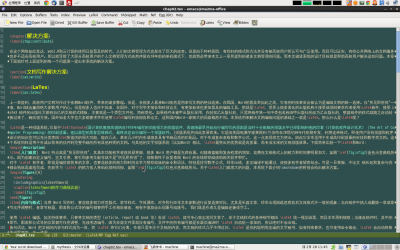
\includegraphics{latexsource}
  \caption{LaTeX源文件}
  \label{fig:xfig6}
\end{figure}

\subsection{\smarkdown}
\label{sec:smarkdown}

\smarkdown是什么,其实它是本文作者自己起的名字,可以理解成science Markdown 或者 scholar Markdown的缩写。其实就是一个扩展版本的Markdown标记语言。首先还是简单介绍一下Markdown标记语言:

简单来说,Markdown 其实是一种轻量级的标记语言。或者说,它规定了一些文本的书写格式。

它实际上是个非常简单、非常容易学习的语法。这个语法简单到每个人都可以在5分钟以内学会。更重要的是,Markdown语法所有要素,是与写作的习惯一脉相承的,套用句俗语“仅为写作而生”。

Markdown诞生于互联网时代,更是由深谙互联网文本之道的John Gruber等人设计。因为Ruby与github\footnote{是一个用于使用Git版本控制系统项目的共享虚拟主机服务。它由GitHub公司(曾称Logical Awesome)的开发者Chris Wanstrath、PJ Hyett和Tom Preston-Werner使用Ruby on Rails编写而成}圈的极客们的热捧,以及来自github、Stackoverflow等的大力支持。从一开始,就建立一个完整的生态链。可以这么说,Markdown之所以在近些年如此流行是和互联网以及web 2.0的普及分不开的。因为人们习惯于在网络上写博客,写微博,写云端笔记,才有了对于更好更便捷的表达自己想法的工具的诉求。也就是要求既可以方便的显示文本的内容也可以很容易的控制文本的样式。下面简单演示一下Markdown的效果:

\begin{bframe}
  \noindent 
  标题\\
  ==============\\
  附标题\\
  -----------\\
  开始书写正文吧\\
  当然也可以用 *列表* 的形式:\\
  1.   列表项目\\
  2.   还是列表项目\\
\end{bframe}
{\noindent 查看时的效果:}
\begin{bframe}
  \noindent
  {\erhao 标题}\\
  {\sanhao 附标题}\\
  开始书写正文吧\\
  当然也可以用 {\bfseries 列表} 的形式:
  \begin{enumerate}
  \item 列表项目
  \item 还是列表项目
  \end{enumerate}
\end{bframe}
很显然,Markdown用很简单好记的标记就能实现一般情况下的文本格式排版,一切就这么简单。Markdown之所以在被鼓吹之后,越来越流行,不是因为它复杂,而是因为它足够简单。

Markdown虽然使用简单,但是其语法中只定义了日常排版最常用的一些情况,比如标题、段落、列表、强调、贴图等。缺乏一些我们科技排版中必要的元素,比如:表格、参考文献、脚注等。这也正是本文作者要对其进行扩展的原因所在。扩展后的Markdown语法,更加适合科技文献的编写。而且也保留了Markdown语法的简洁性,可以很快掌握。关于具体的Markdown语法和扩展后的\smarkdown语法,本文将在下面系统实现的章节详细介绍。

\subsection{Smarkdown+LaTeX}
\label{sec:sandl}

\smarkdown就像流行音乐,简单易学,通俗易懂,可以被大多数人所接受。\LaTeX就像古典音乐,优雅灵活,高深强大,但是不是很容易被大多数人所接受。没有任何编程基础的人要想上手使用\LaTeX,并不是一件很容易的事情,起码需要一个多星期的系统学习\footnote{这个时间没有做广泛调研,可能因人而异},即使这样也不能完全掌握要领。但是学习使用\smarkdown却只需短短几分钟,就可以掌握它的所有的语法,并开始编辑工作,而且编辑过程中可以一直专注与文章的内容。图~\ref{fig:xfig7}描述了不同文档规模下\LaTeX、\smarkdown、Word编辑文档时,耗费在排版格式上的精力的比较。可以看出\smarkdown不仅对于小规模的文档简单易学,而且随着文档规模的增大,用户用于排版的精力并没有太大的增加。
\begin{figure}[H]
  \centering
  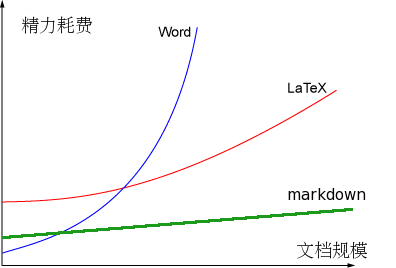
\includegraphics{latexmarkdownword}
  \caption{LaTeX,Smarkdown,Word精力耗费比较}
  \label{fig:xfig7}
\end{figure}
那么,如果把这两个工具结合起来,使用\smarkdown作为给一般用户前端编辑工具,使用\LaTeX作为编辑后生成最终PDF文档的工具。那么就等于把一个复杂而又强大的东西简单化了。相当于在普通用户与\LaTeX专业排版直接架构了一座沟通的“金桥”。用户可以在系统提供的编辑页面编写\smarkdown格式的文章,当然由于\smarkdown可以及时的翻译成html格式,所以用户可以在第一时间看到自己的文档的最终样式\footnote{由于系统允许插入LATEX语法片段,所以这里的预览并不完全是最终格式}。然后系统提供各种\LaTeX的模板供用户使用,其中有个大学的学位论文模板,个出版社的期刊论文模板,通过这些模板,用户可以把自己的文章导出为套用任意模板的最终格式的PDF文件。当然高级用户亦可下载系统转换好的\LaTeX格式的文件,在用自己的模板生成最终文件。而且编辑页面中可以插入\LaTeX语法片段,这些特性可以给那些熟悉\LaTeX的高级用户使用,以生成高质量的数学公式,化学式等。

以上所描述的就是本系统应对高校用户在文档编辑中遇到问题的解决方案:\fbox{ \smarkdown的前端编辑和\LaTeX的后台处理}。当然,要实现这些需要做很多工作,比如首先要实现一个可以把\smarkdown翻译成\LaTeX的编译器,我们将在下面系统实现的章节对这些做详细的描述。


\section{文档存储解决方案}
\label{sec:save}

上一章提到,高校用户个人文档保存存在严重的安全隐患和效率问题。主要体现在:
\begin{itemize}
\item 文档保存介质安全性低,文档有丢失风险。
\item 文档保存位置繁多,互相同步困难,管理混乱。
\item 缺乏必要的版本控制与备份机制。
\item 缺乏文档的标签(关键字)管理,和全文查找,查找和管理困难。
\item 多人协作的项目文件,保存与管理混乱。
\end{itemize}
其实高校用户遇到的这些问题在广大使用计算机办公的用户中也是很普遍的问题。早些年,在网络还没有达到今天如此发达与普及的时候,这些问题一直困扰着使用计算机进行办公的人们了。直到近两年,随着网络的普及,web2.0和云计算的流行,逐渐的出现了一些解决以上这些问题的解决方法。比如最近非常流行的各种云笔记服务,网络磁盘,github等。
\begin{itemize}
\item 云笔记是一款跨平台的简单快速的个人记事备忘工具,操作界面简洁高效。会议记录、日程安排、生活备忘,奇思妙想、快乐趣事以及任何突发灵感都可快速记录到云笔记,更支持拍照和添加图片作为笔记附件。目前比较常用的有evernote,有道云笔记等。
\item 网盘,又称作网络U盘、网络硬盘,是由不同网络公司推出的在线存储服务。向用户提供文件的存储、访问、备份、共享等文件管理等功能,用户可以把网盘看成一个放在网络上的硬盘或U盘,不管你是在家中、单位或其它任何地方,只要你连接到因特网,你就可以管理、编辑网盘里的文件。不需要随身携带,更不怕丢失。目前常用的有百度云盘,新浪微盘等等。
\item GitHub可以托管各种git\footnote{一个分布式的版本控制系统,最初由Linus Torvalds编写,用作Linux内核代码的管理。在推出后,Git在其它项目中也取得了很大成功。}库,并提供一个web界面,它的特点在于提供完善的分布式版本控制机制,而且从另外一个项目进行分支的简易性。
\end{itemize}
通过以上介绍,可以发现对于文档的保存,管理,多设备同步,版本控制这些问题,在网络时代已经有了很完备的解决方案,而且从其发展的速度来看,文档的网络存储模式将逐渐的取代本机存储模式,成为未来文档存储的主要方式。

但是,这些社会上流行的文档管理服务真的适合我们高校用户的需求吗?下面列举几条高校用户使用这些服务遇到的典型问题:
\begin{description}
\item[网络速度与费用问题] 众所周知,高校中使用最为广泛的网络是教育网,而教育网和公共网络\footnote{以电信和联通为主}之间的通信带宽一直很低。直观的感受就是教育网访问架设在公共网络上的服务会非常缓慢。而大部分云文档服务都架设在公共网络上。在网络速度得不到保证的情况下,用户体验可以说并不好。

  这还不是问题的全部,教育网中普遍存在按流量收费的情况,从公网服务中获取的文件如果很大,那么用户可能会为此付出高额的网络流量费用\footnote{据了解,大多数高校并不会让老师和学生自己承担此费用,而是由学校统一承担。但是也有个别高校依然收取高额网络流量费用。}。
\item[数据安全问题] 高校用户和社会用户的最大区别是,高校用户要存储的文档,大多是个人的成果和项目文档这样的学术性文档。这就涉及到很大一部分文档需要保密,甚至有个别的军工项目的文档几乎是绝密等级的。虽然很多云平台声称他们的存储是严格加密的,数据安全不存在问题。但是这些平台毕竟是商业平台,他们的开发和维护者也是抱有商业目的的公司。显然,把高校用户的这些具有很高商业价值的文档放置于这些平台上,安全性确实很难让人放心。
\item[流行未必长久] 刚才说过,商业平台台毕竟是是抱有商业目的的公司在维护,公司的目的自然是盈利。目前云服务概念如此流行。以至于提供云服务的公司如雨后春笋纷纷涌现出来。也许在不久的将来,云服务不再想今天这样流行,那时这些公司还能像今天这样提供如此稳定与完备的服务吗?甚至有些公司是否还存在也要打上一个大大的问号。“皮之不存毛将焉附“,那时,我们的文档的命运就可想而知了。
\item[缺少一站式服务] 上面提到的各种云服务平台,虽然都各具特点,但是每一个也没有提供一个完整的解决方案。
\end{description}
综上所述,当今虽然有很多既有的云服务可以解决高校用户文档管理问题。但是由于种种原因,高校用户使用这些服务依然存在很多障碍。这也给本系统的设计和实现提供了必要性,下面介绍一下本系统的解决方案:
本系统应对高校用户在文档保存中遇到问题的解决方案:\fbox{基于网络存储模式的云服务}。服务的基本模式类似于“云笔记”与“网盘”的结合,同时提供最基本的版本控制功能。每个用户的文档保存在网络云端的服务器上,系统为每个用户提供一定额度的磁盘空间,用户既可以在系统中使用纯文本的方式编写自己的文档,也可以把即有的Word,Excel等格式的文档上传到系统中。而且系统支持web方式、客户端程序方式、移动客户端方式(android,ios)的访问支持。也就是说,用户可以在任何一个可以上网的电脑,手机或者平板电脑上访问和管理自己的文件。而且而且每个设备上的文档都自动同步。避免了不同设备中文档版本冲突的问题。不仅如此,由于本系统服务器将架设在学校图书馆\footnote{本项目为图书馆学术支撑计划之一}。所以从网络服务角度其具有如下优势:
\begin{itemize}
\item 图书馆拥有自己的专业机房,和完备的磁盘阵列设备和备份策略,保证了用户的文档保存在安全的介质上,不用由于硬件的损坏而导致文档的丢失。%图~\ref{fig:xfig8}为图书馆机房中磁盘阵列照片。
\item 图书馆机房为学校校园网的重要节点,拥有校园网内的超高网速。用户使用系统不会有明显的延时感。操作网络文件的效率几乎可以和操作本地文件相似。
\item 图书馆为非盈利性机构,为学校的师生服务是它的职责。不会因为某些商业因素而导致服务质量的降低,而且随着系统使用量的增大,学校投入的增加,服务的性能和存储量将逐年递增。
\item 图书馆有大量的文献资源和富有经验的人力资源,可以在系统中为师生提供高质量的文档管理服务,比如:文档信息补全,成果认证,文献获取等服务。
\end{itemize}
% \begin{figure}[H]
%   \centering
%   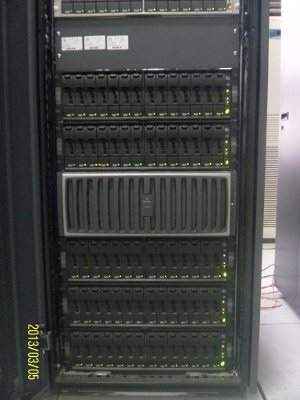
\includegraphics{raiddisk}
%   \caption{磁盘阵列}
%   \label{fig:xfig8}
% \end{figure}

\section{文档分发解决方案}
\label{sec:giveout}

以上的解决方案基本上围绕着个人管理文档这个主题,解决的问题也主要是用户个体在文档的建立和保存方面遇到的困难。但是有些时候,用户并不满足于编辑并保存好自己的文档,他们需要把文档分享给别人,和其他人一起合作完成文档,或者和他人就一篇文档展开交流。上文也提到了,当今高校中的文档分发方式还处于比较原始的阶段,基本上以电子邮件,qq为主。不仅操作繁琐,而且安全性很低。
\section{个人成果展示方案}
\label{sec:display}

\section{项目管理解决方案}
\label{sec:project}




